% Author: Dr. Matthias Jung, DL9MJ
% Year: 2020
\documentclass[convert = false, border=5pt]{standalone}
\usepackage{fontspec}
\setmainfont{Roboto}
\usepackage[siunitx, straightvoltages, europeanresistors, european inductor]{circuitikzgit}
\usepackage{tikz}


\usepackage[siunitx, straightvoltages]{circuitikzgit}
\usepackage{amsmath}
\usepackage{unicode-math}
\setmathfont{Fira Math}
\setmathfont[range=up]{Roboto}
\setmathfont[range=it]{Roboto-Italic}
\setmathfont[range=\int]{Fira Math}
\usepackage[euler]{textgreek}
\usepackage{pgfplots}
\pgfplotsset{compat=1.8}
\usepackage{mathtools}
\usepackage[utf8]{inputenc} % UTF8 encoding
\usepackage{tikz}

\begin{document}

\pgfplotsset{every axis plot}
%\pgfplotsset{grid style=dotted}
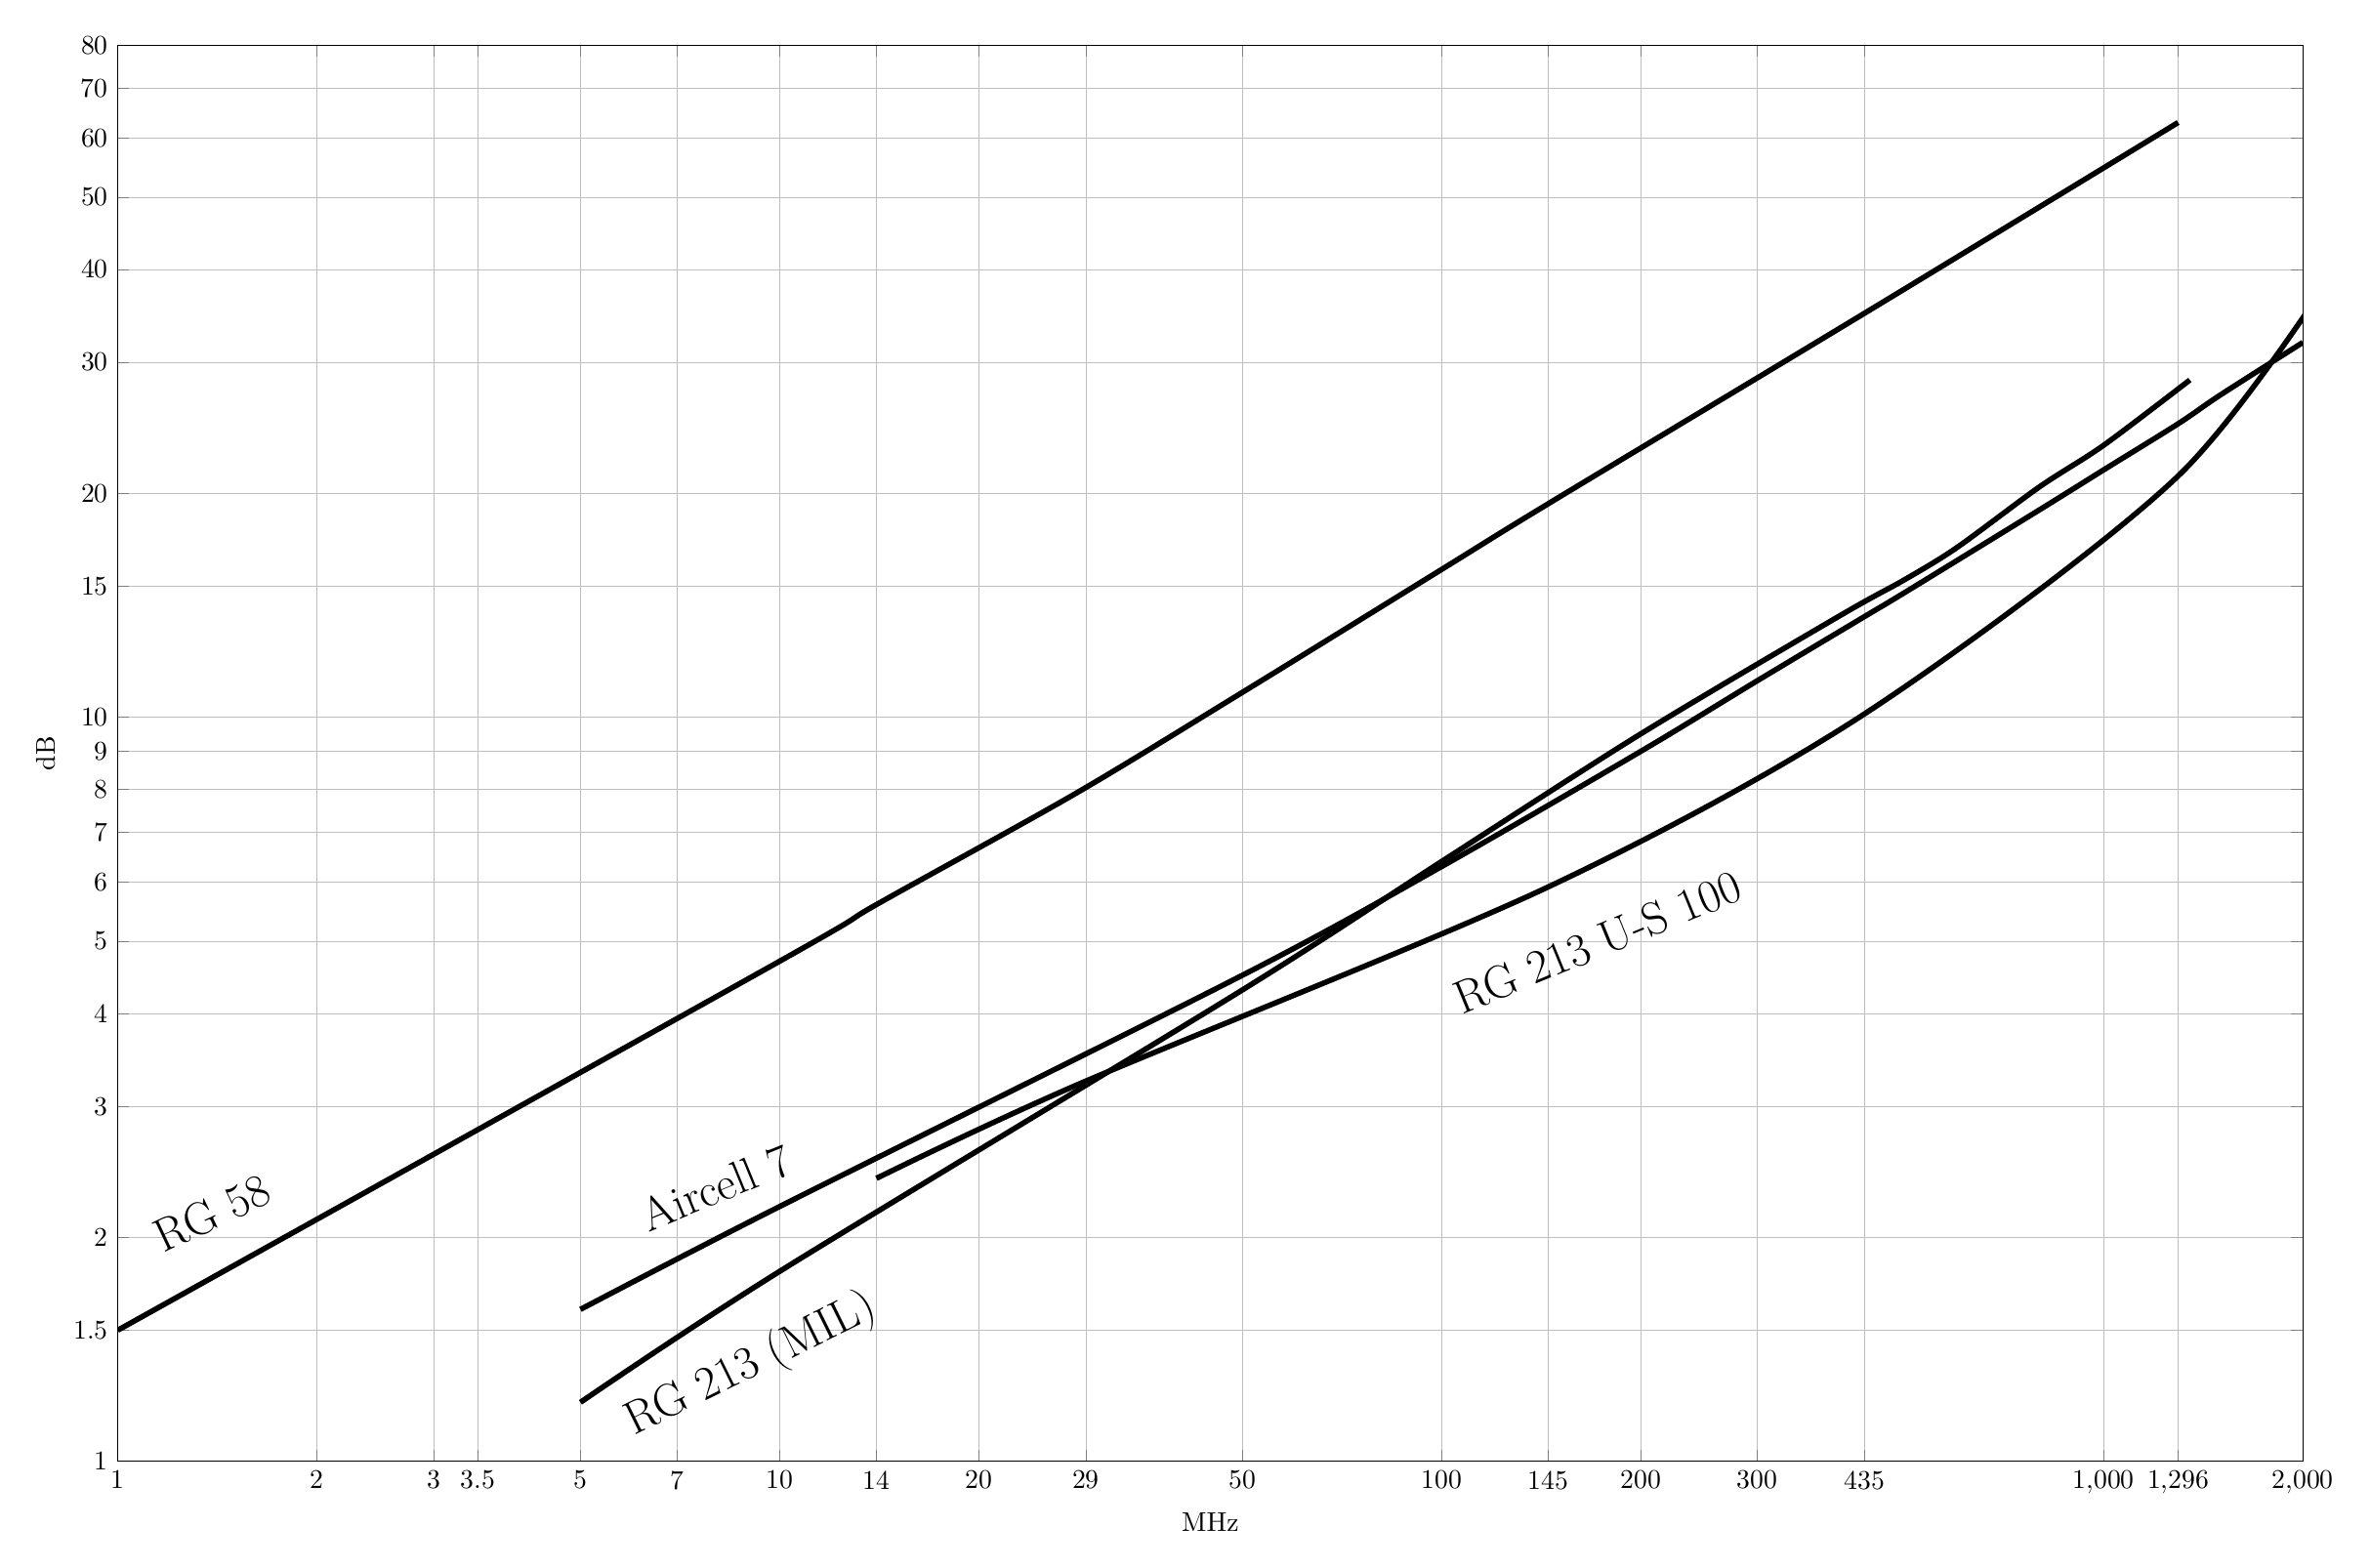
\begin{tikzpicture}
\begin{loglogaxis}
    [clip marker paths=true,legend cell align=left,
    legend style={
        at={(0.5,-0.2)},
        anchor=north},
    width=30cm,
    %height=30cm,
    height=20cm,
    legend columns=2,
    xlabel=MHz,
    ylabel=dB,
    xmin=1, xmax=2000,
    ymin=1, ymax=80,
    %ymin=1e-1, ymax=300,
    xtick={1,2,3,3.5,5,7,10,14,20,29,50,100,145.0,200.0,300.0,435.0,1000.0,1296.1,2000.1},
    ytick={0.1,0.2,0.3,0.4,0.5,0.6,0.7,0.8,0.9,1,1.5,2,3,4,5,6,7,8,9,10,15,20,30,40,50,60,70,80,90,100,200,300},
    yticklabel style={/pgf/number format/.cd,fixed,precision=1},
    xticklabel style={/pgf/number format/.cd,fixed,precision=1},
    xticklabel={%
      \pgfmathfloatparsenumber{\tick}%
      \pgfmathfloatexp{\pgfmathresult}%
      \pgfmathprintnumber{\pgfmathresult}%
    },
    yticklabel={%
      \pgfmathfloatparsenumber{\tick}%
      \pgfmathfloatexp{\pgfmathresult}%
      \pgfmathprintnumber{\pgfmathresult}%
    },
    grid=major,
    grid style={line width=.1pt, draw=gray!10},
    major grid style={line width=.2pt,draw=gray!50},
    ]

    % https://kabel-kusch.de/Datenblatt.htm
    \addplot[smooth, line width=2pt] coordinates
    {(   1,1.5)
     (  10,4.7)
     (  14,5.6)
     (  28,7.9)
     (  50,10.8)
     ( 100,15.8)
     ( 144,19.3)
     ( 435,34.9)
     (1296,63.0)
     %(2000,80.0)
     };
    \node[rotate=25.3] at (axis cs:1.8, 2.2) [anchor=south east] {\LARGE{RG 58}};
     
    %http://www.dd1us.de/Downloads/Daten%20Koaxialkabel.pdf
    \addplot[smooth, line width=2pt] coordinates
    {(  14,2.4)
     (  28,3.2)
     ( 144,5.9)
     ( 435,10.1)
     (1296,21.1)
     (2320,42)
     };
    \node[rotate=22.3] at (axis cs:300, 5.6) [anchor=south east] {\LARGE{RG 213 U-S 100}};

    %https://www.classicinternational.de/antennen-montage/kabel-koax-audio-steuer/koaxkabel/rg-213-u-mil-c17f/
    \addplot[smooth, line width=2pt] coordinates
    {(  5,1.2)
     (  10,1.8)
     (  50,4.3)
     ( 100,6.4)
     ( 200,9.5)
     ( 400,13.7)
     ( 500,15.3)
     ( 600,16.9)
     ( 800,20.4)
     (1000,23.2)
     (1350,28.4)
     };
    \node[rotate=26.3] at (axis cs:15, 1.5) [anchor=south east] {\LARGE{RG 213 (MIL)}};

    %https://kabel-kusch.de/Koaxkabel/Aircell-7/AIRCELL-7.htm
    \addplot[smooth, line width=2pt] coordinates
    {(  5,1.6)
     (  10,2.2)
     (  50,4.5)
     ( 100,6.3)
     ( 200,9.0)
     ( 300,11.2)
     ( 432,13.6)
     ( 500,14.7)
     ( 800,19.0)
     (1000,21.5)
     (1296,24.8)
     (1500,27.1)
     (2000,31.9)
     };
    \node[rotate=22.3] at (axis cs:11, 2.4) [anchor=south east] {\LARGE{Aircell 7}};

\end{loglogaxis}
\end{tikzpicture}

\end{document}

